%%%%%%%%%%%%%%%%%%%%%%%%%%%%%%%%%%%%%%%%%%%%%%%%%%%%%%%%%%%%%%%%%%%%%%
% Presentación: Registración de imágenes médicas 2D
% Día: 15/06/17
%
% Autor: Ariel Hernández
% e-mail: ariel.h.estevenz@ieee.org | ahernandez@cae.cnea.gov.ar
% Comisión Nacional de Enería Atómica
%
%%%%%%%%%%%%%%%%%%%%%%%%%%%%%%%%%%%%%%%%%%%%%%%%%%%%%%%%%%%%%%%%%%%%%%

\documentclass{beamer} %
\usetheme{CambridgeUS}
\usepackage[utf8]{inputenc}
\usefonttheme{professionalfonts}
\usepackage{times}
\usepackage{tikz}
\usepackage{amsmath}
\usepackage{verbatim}
\usetikzlibrary{arrows,shapes}

\author{}

\institute{CNEA}
\date{15/06/2017}

\title[Registración de imágenes]{Registración de imágenes médicas en 2D}
\author[Ariel Hernández]{\small Ariel Hernández}
\institute[]{\large CNEA\\
\footnotesize División Sistemas Digitales y Robótica\\
\small Subgerencia de Instrumentación y Control}
\date{15/06/2017}

\begin{document}

\begin{comment}
:Title: Registración de imágenes médicas
:Tags: registración, imágenes, 2D, mutual information, BNCT, PET, CT
:Use page:
\end{comment}

\tikzstyle{every picture}+=[remember picture]
\everymath{\displaystyle}

% Frame 0
\begin{frame}

\titlepage

\begin{tabular}{l}
  \includegraphics[width=3.5cm]{images/logos/CNEA_logo.png}
\end{tabular}

\end{frame}

% Frame 1
\begin{frame}
\frametitle{AR-PET}
\tikzstyle{na} = [baseline=-.5ex]

ARPET: Tomógrafo por emisión de positrones

  \begin{tabular}{cl}
     \begin{tabular}{c}
       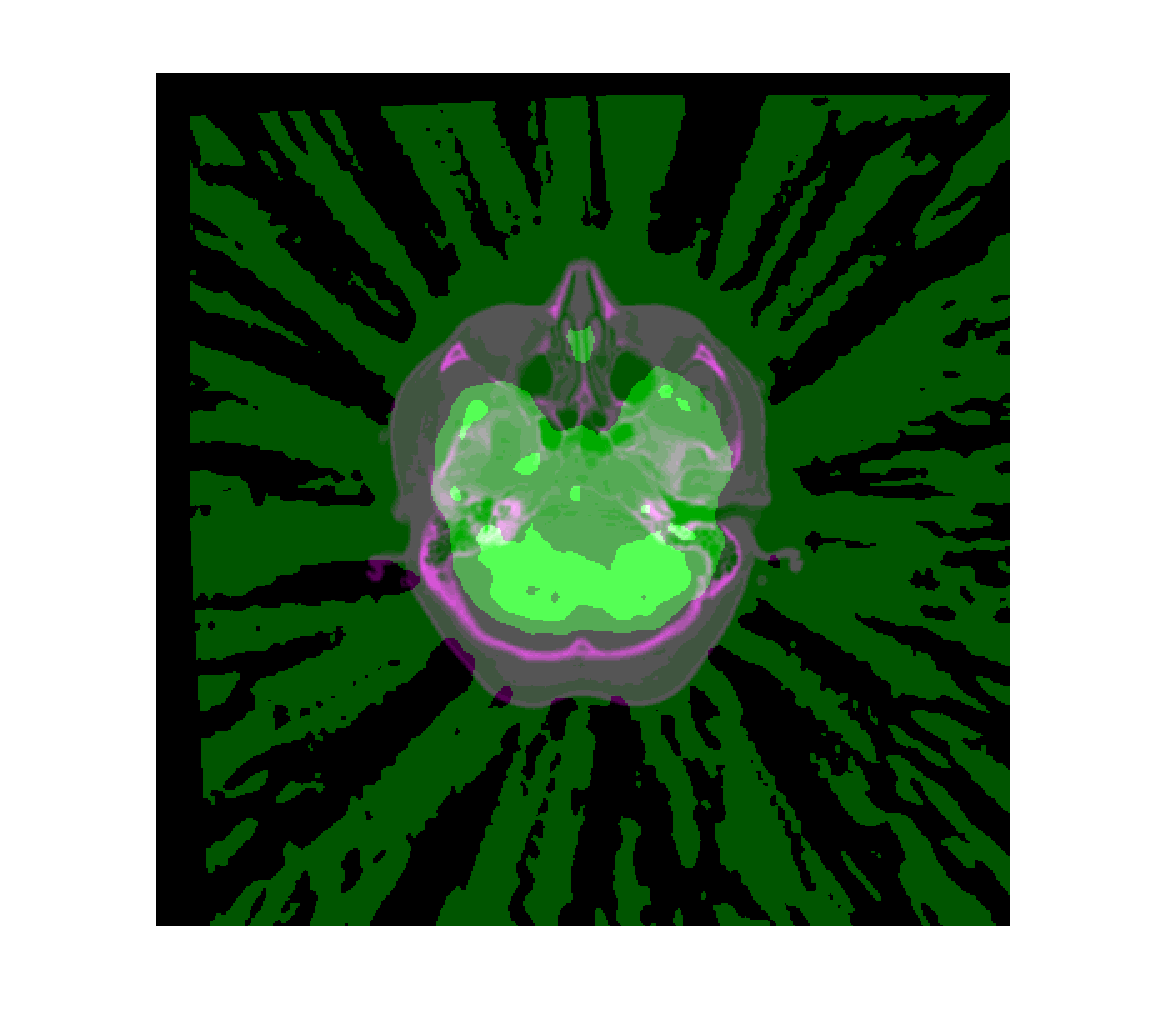
\includegraphics[height=5cm, width=3.5cm]{images/7-reg.eps}
     \end{tabular}
   & \begin{tabular}{l}
       \parbox{0.5\linewidth}{
        \begin{itemize}
        \pause
        \item Equipo desarrollado en el país
        \pause
        \item Para la detección utiliza seis cámaras gamma
        \pause
        \item Cada cámara contiene un cristal continuo Yoduro de Sodio (NaI)
        \pause
        \item No tiene CT
        \end{itemize}
        }
    \end{tabular}  \\
  \end{tabular}
\end{frame}

% Frame 2
\begin{frame}
\frametitle{IR: Monomodal y Multimodal}
\framesubtitle{Características de las imágenes}

\begin{itemize}
\pause
\item Fueron adquiridas en distinto tiempo.
\pause
\item Provienen de distintos dispositivos de diagnóstico
\pause
\item Se adquirieron desde diferentes ángulos
\end{itemize}

\end{frame}

% Frame 3
\begin{frame}
\frametitle{IR: Monomodal y Multimodal}
\framesubtitle{Tipo de registración}

\begin{itemize}
\pause
\item Monomodal
\pause
\item Multimodal
\end{itemize}

\end{frame}

% Frame 4
\begin{frame}
\frametitle{IR: Monomodal y Multimodal}
\framesubtitle{Denominación de las imágenes}

\begin{itemize}
\pause
\item Imagen objetivo o detectada, en inglés \textit{moving}
\pause
\item Imagen referencia o fuente, en inglés \textit{rigid}
\end{itemize}

\end{frame}

% Frame 5
\begin{frame}
\frametitle{Etapas en IR: Espacio de características}

Características elegidas en la imagen:

\pause
\begin{itemize}
\item Valor del pixel
\item Información del contorno
\item Información de picos de objetos
\item etc.
\end{itemize}

\end{frame}

% Frame 6
\begin{frame}
\frametitle{Etapas en IR: Espacio de búsqueda}

Tipo de transformación:

\pause
\begin{itemize}
\item rígidas o \textit{rigid}
\item afín o \textit{affine}
\item no rígidas
\end{itemize}

\end{frame}

% Frame 7
\begin{frame}
\frametitle{Etapas en IR: Estrategia de búsqueda}

Mecanismo para la elección de las sucesivas transformaciones.

\pause
\begin{itemize}
\item \textit{hill climbing}
\end{itemize}

\end{frame}

% Frame 8
\begin{frame}
\frametitle{Etapas en IR: Medida de similitud}

Mecanismo de cuantificación de las diferencias geométricas entre ambas imágenes.

\pause
\begin{itemize}
\item Correlación
\item Error Cuadrático Medio
\item Información Mutua.
\end{itemize}

\end{frame}

% Frame 9
\begin{frame}
\frametitle{IR: Insight Journal Database}
\includegraphics[height=6cm, width=12cm]{images/IJD.png}
\end{frame}

% Frame 10
\begin{frame}
\frametitle{IR: Registración en ARPET}

Algoritmo de registración de imágenes 2D

\begin{itemize}
\pause
\item Espacio de características: valor del píxel
\pause
\item Espacio de búsqueda: rígida
\pause
\item Estrategia de búsqueda: \textit{hill climbing} por fuerza bruta
\pause
\item Medida de similitud: Información Mutua.
\end{itemize}

\pause
\begin{block}{}
  Se realiza una transformación de traslación de a 1 pixel hasta completar el tamaño de la imagen y medio grado en la rotación de $-\pi/2$ a $\pi/2$, donde se obtiene una matriz de MI de tamaño 512x512x181, ya que son 512x512 traslaciones por cada rotación.
\end{block}

\end{frame}

% Frame 11
\begin{frame}
\frametitle{IR: Registración en ARPET}

\begin{figure}
  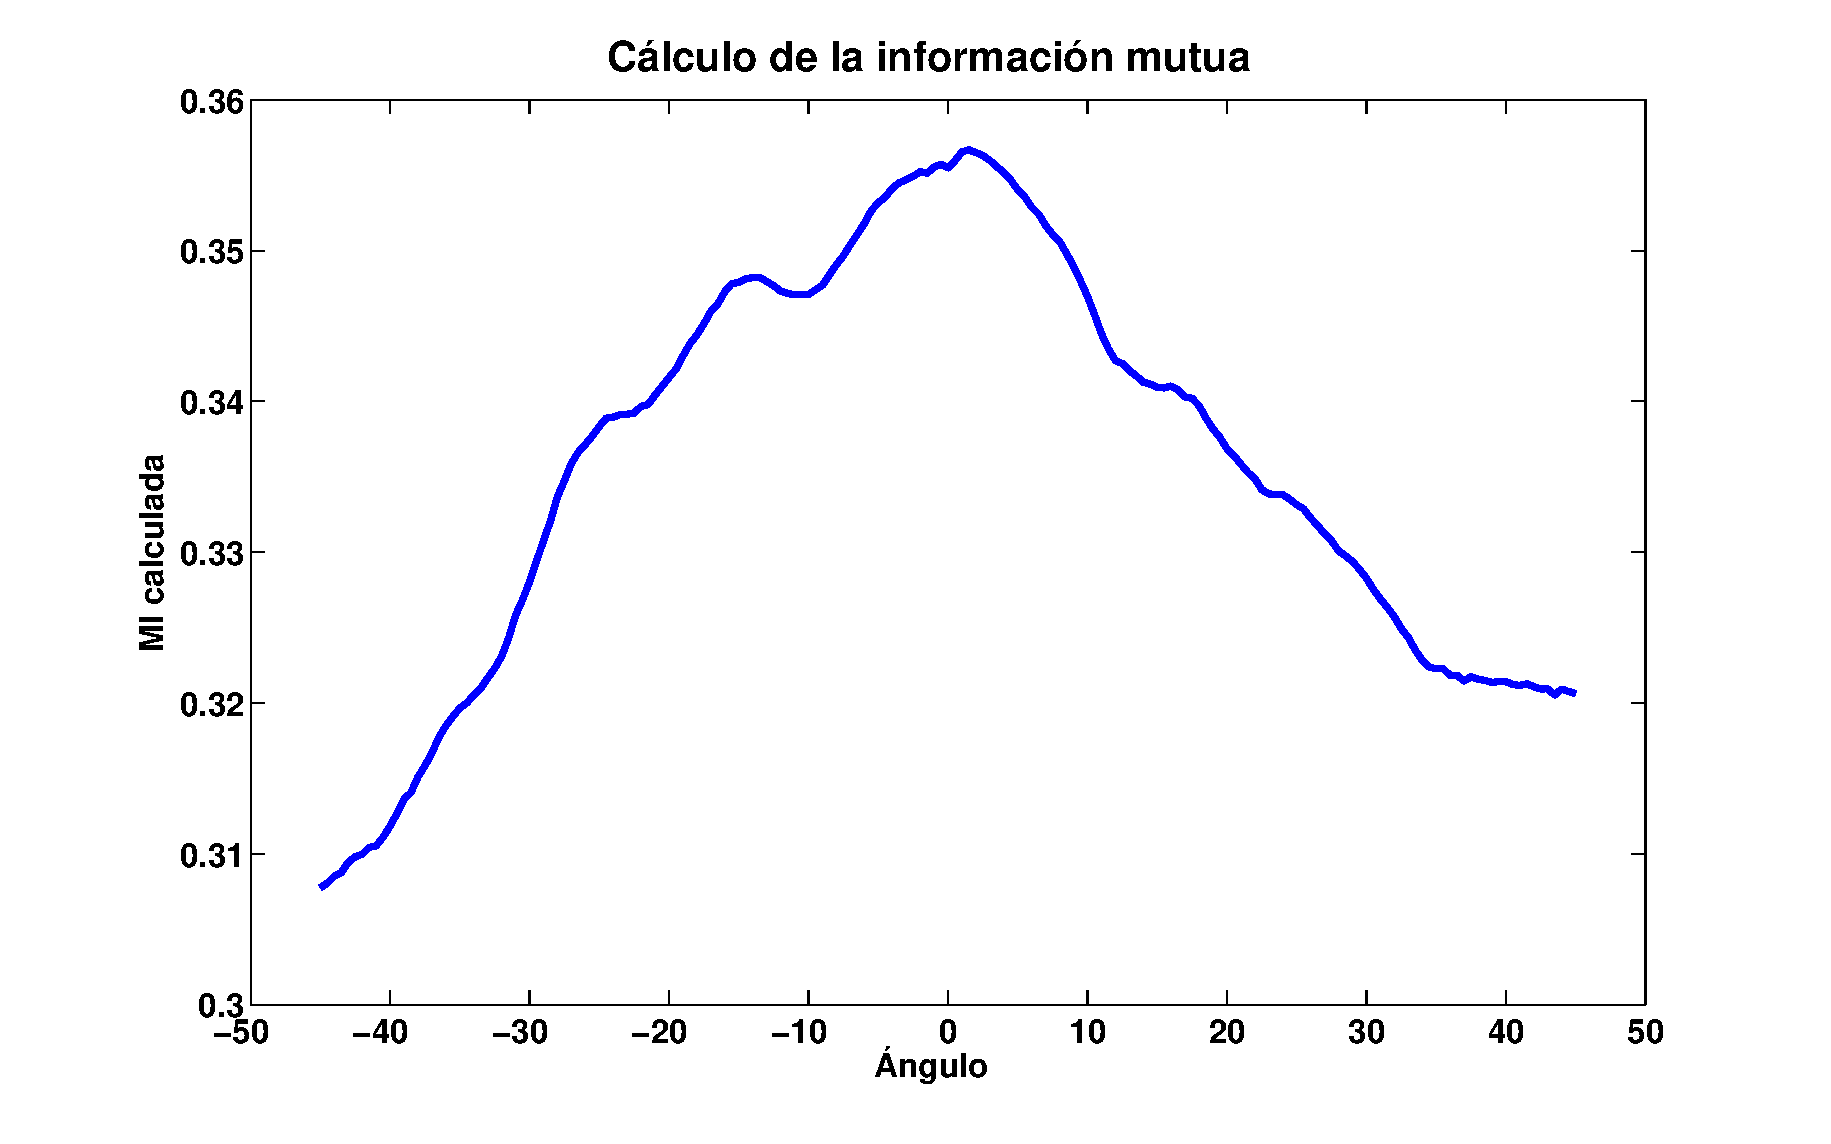
\includegraphics[width=\textwidth]{images/calc_mi_matrix_rotation.eps}
\end{figure}

\end{frame}

\begin{frame}
\frametitle{IR: Registración en ARPET}

\begin{figure}
  \includegraphics[width=\textwidth]{images/calc_mi_matrix_translation.eps}
\end{figure}

\end{frame}

% Frame 12
\begin{frame}
\frametitle{IR: Registración en ARPET}

Algoritmo de registración de imágenes 2D

\begin{itemize}
\pause
\item Espacio de características: valor del píxel
\pause
\item Espacio de búsqueda: rígida
\pause
\item Estrategia de búsqueda: \textit{hill climbing} por Metropolis
\pause
\item Medida de similitud: Información Mutua.
\end{itemize}

\end{frame}

% Frame 13
\begin{frame}
\frametitle{IR: Registración en ARPET}

\begin{columns}[onlytextwidth]
\begin{column}{.5\textwidth}
\begin{figure}
  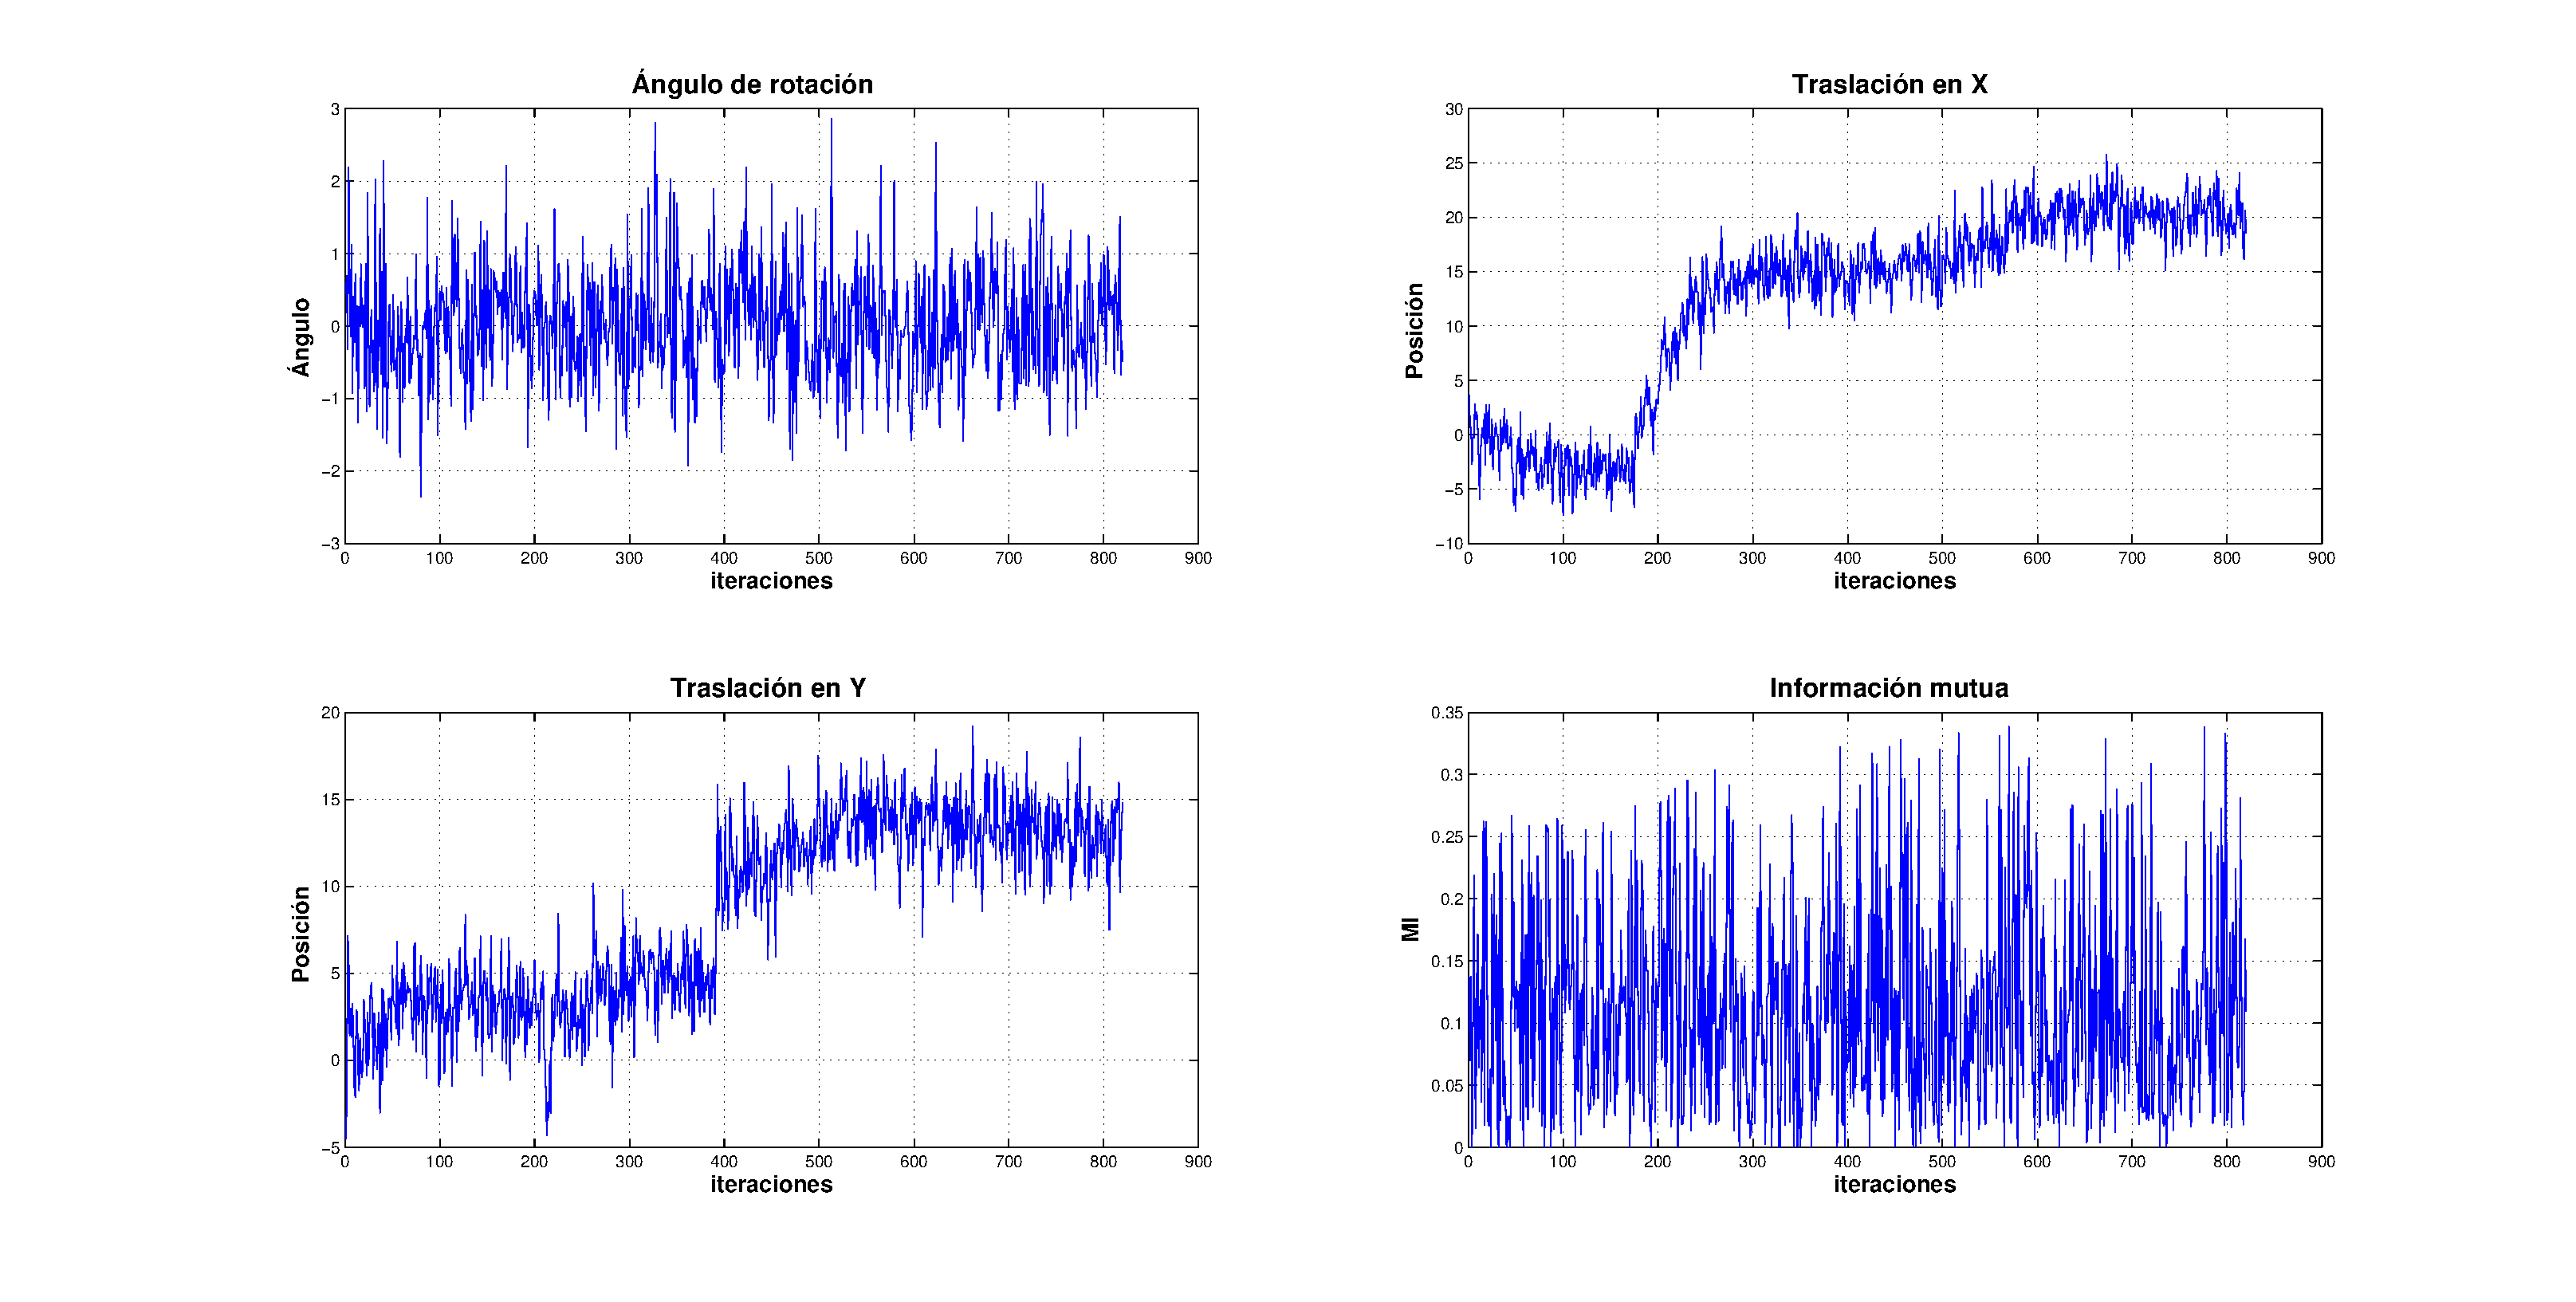
\includegraphics[width=\textwidth]{images/7-all.eps}
  \caption{Todos los parámetros}
\end{figure}
\end{column}
\hfill
\begin{column}{.5\textwidth}
\begin{figure}
  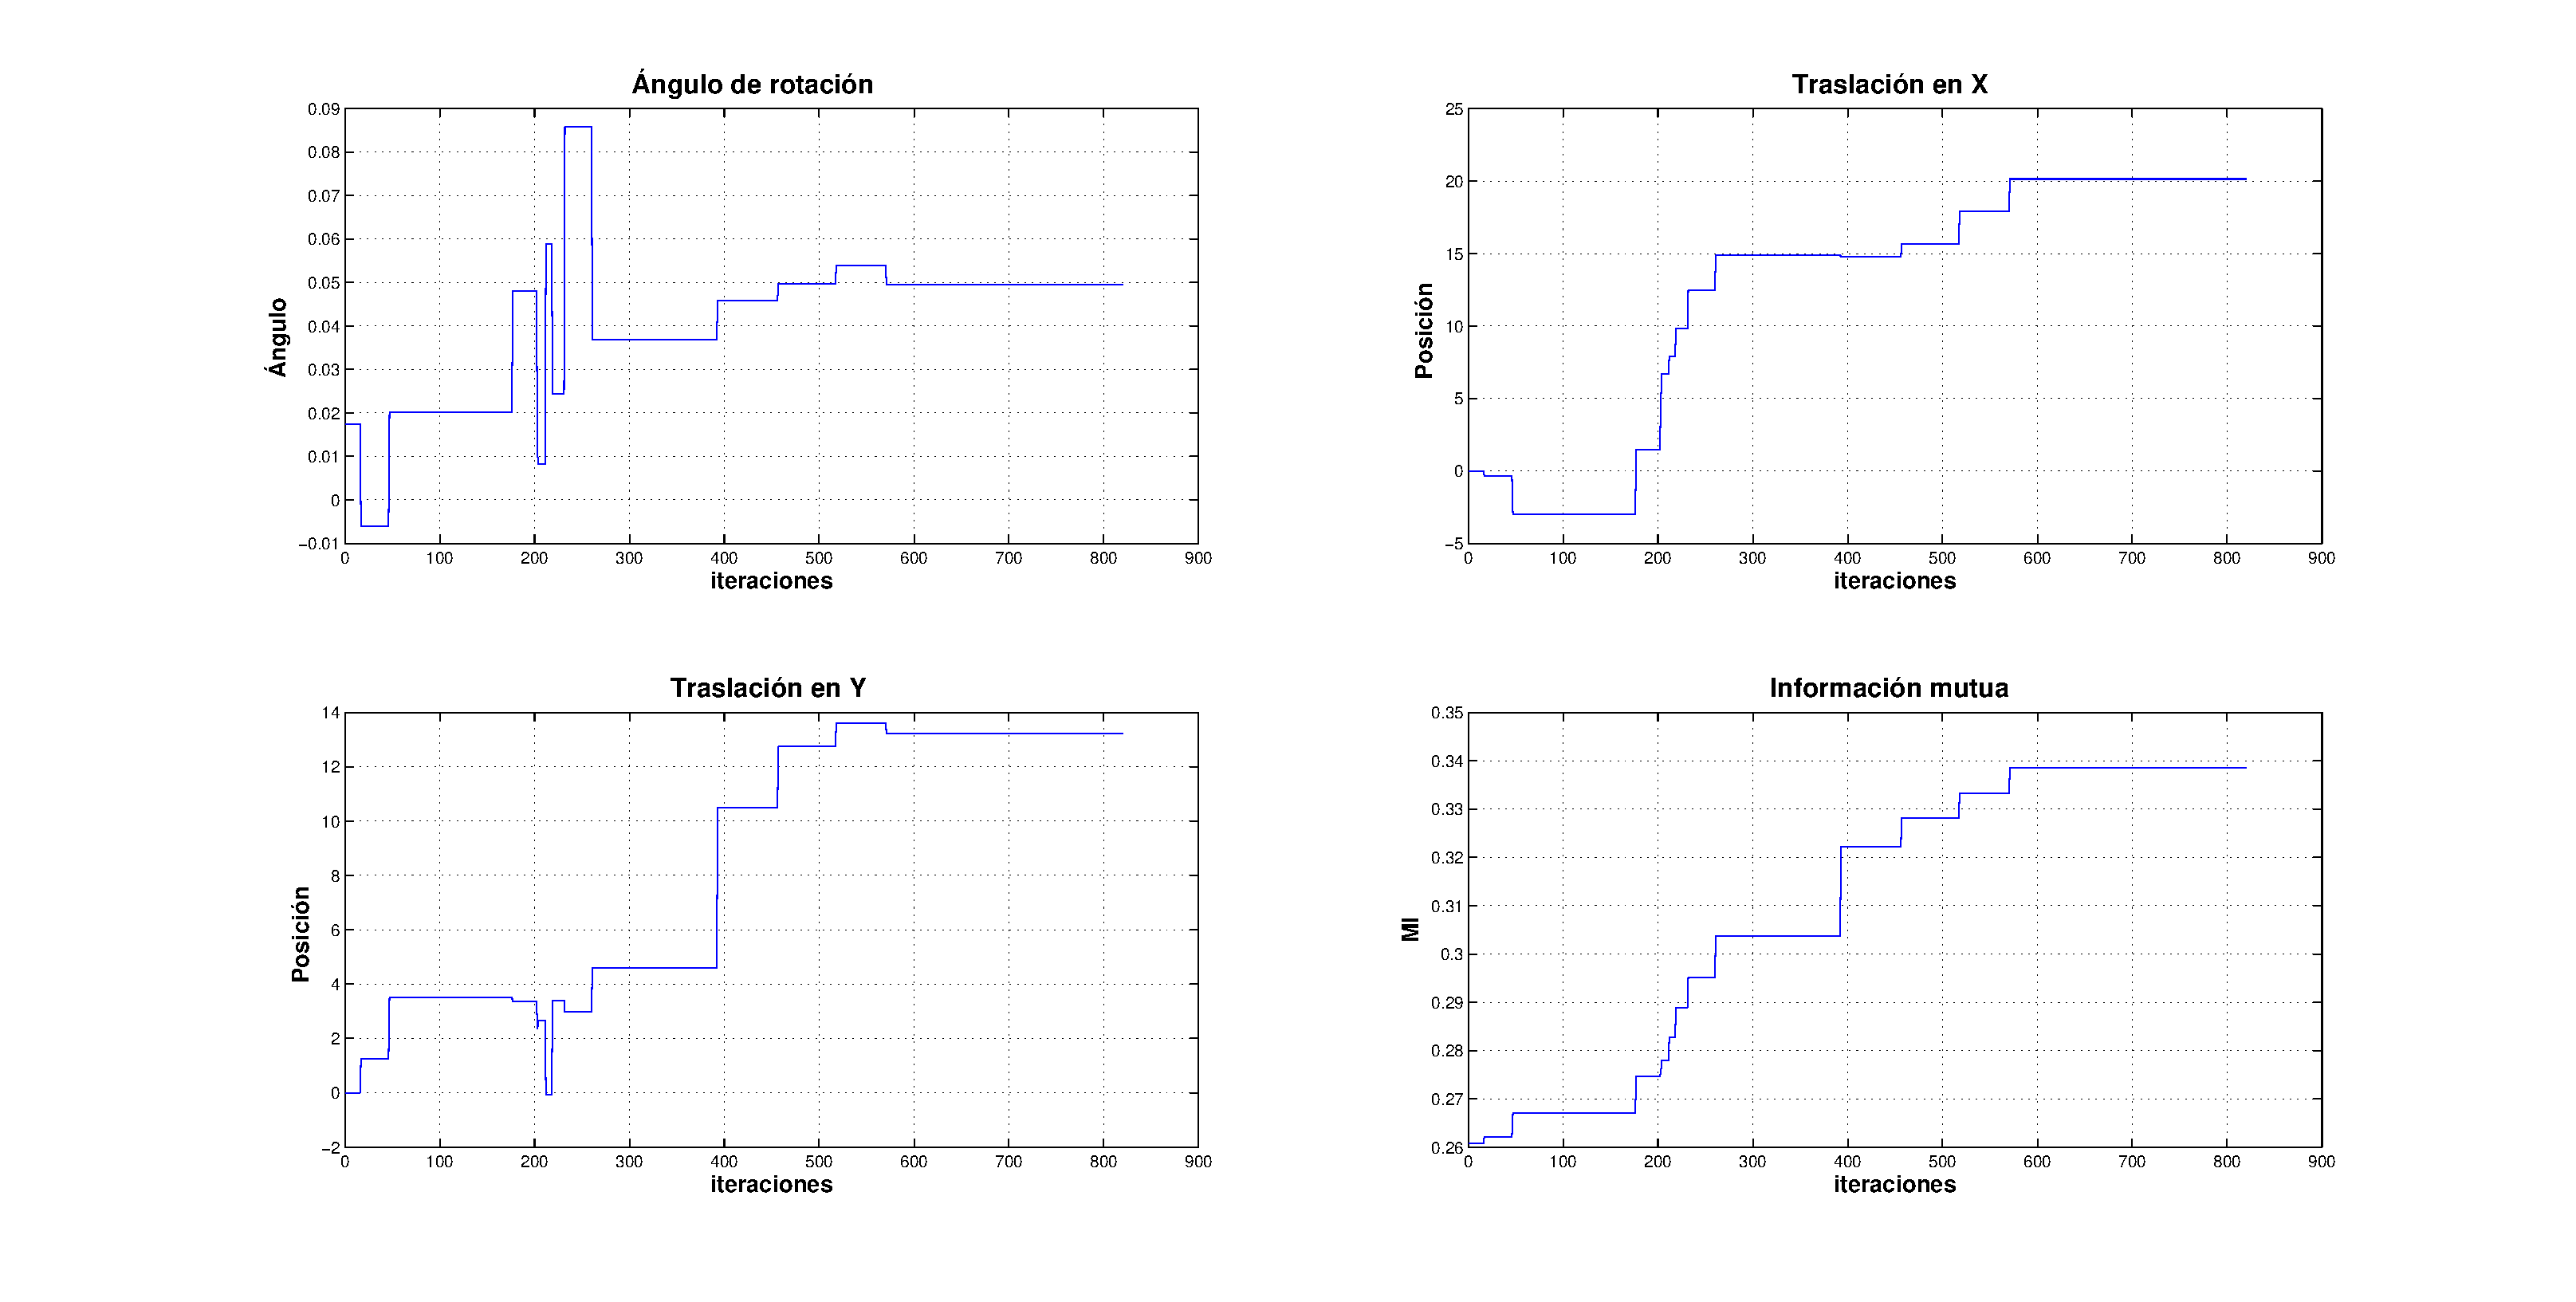
\includegraphics[width=\textwidth]{images/7-accepted.eps}
  \caption{Parámetros aceptados}
\end{figure}
\end{column}
\end{columns}

\end{frame}

% Frame 14
\begin{frame}
\frametitle{IR: Registración en ARPET}

\begin{columns}[onlytextwidth]
\begin{column}{.45\textwidth}
\begin{figure}
  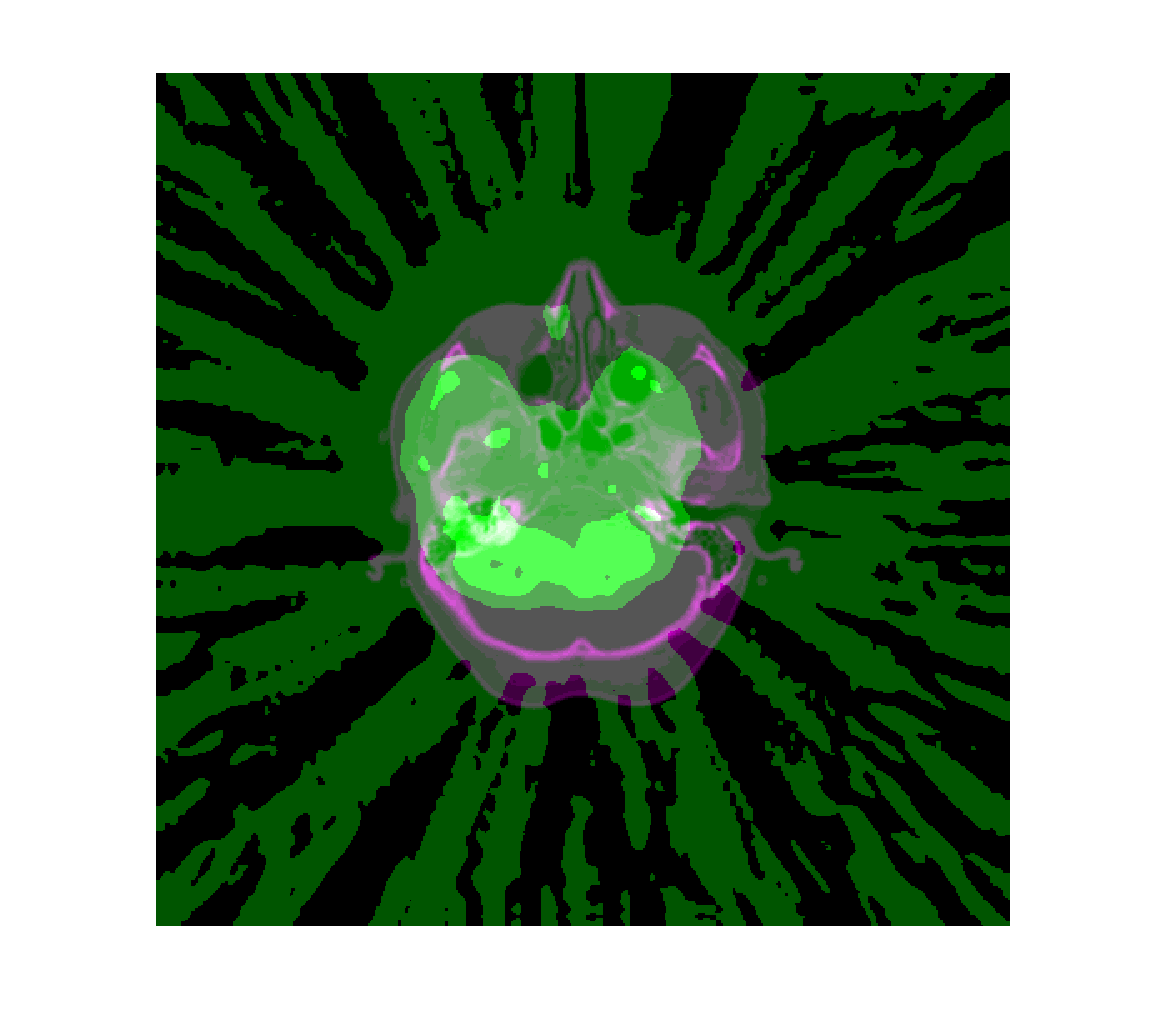
\includegraphics[width=\textwidth]{images/7-unreg.eps}
  \caption{No registradas}
\end{figure}
\end{column}
\hfill
\begin{column}{.45\textwidth}
\begin{figure}
  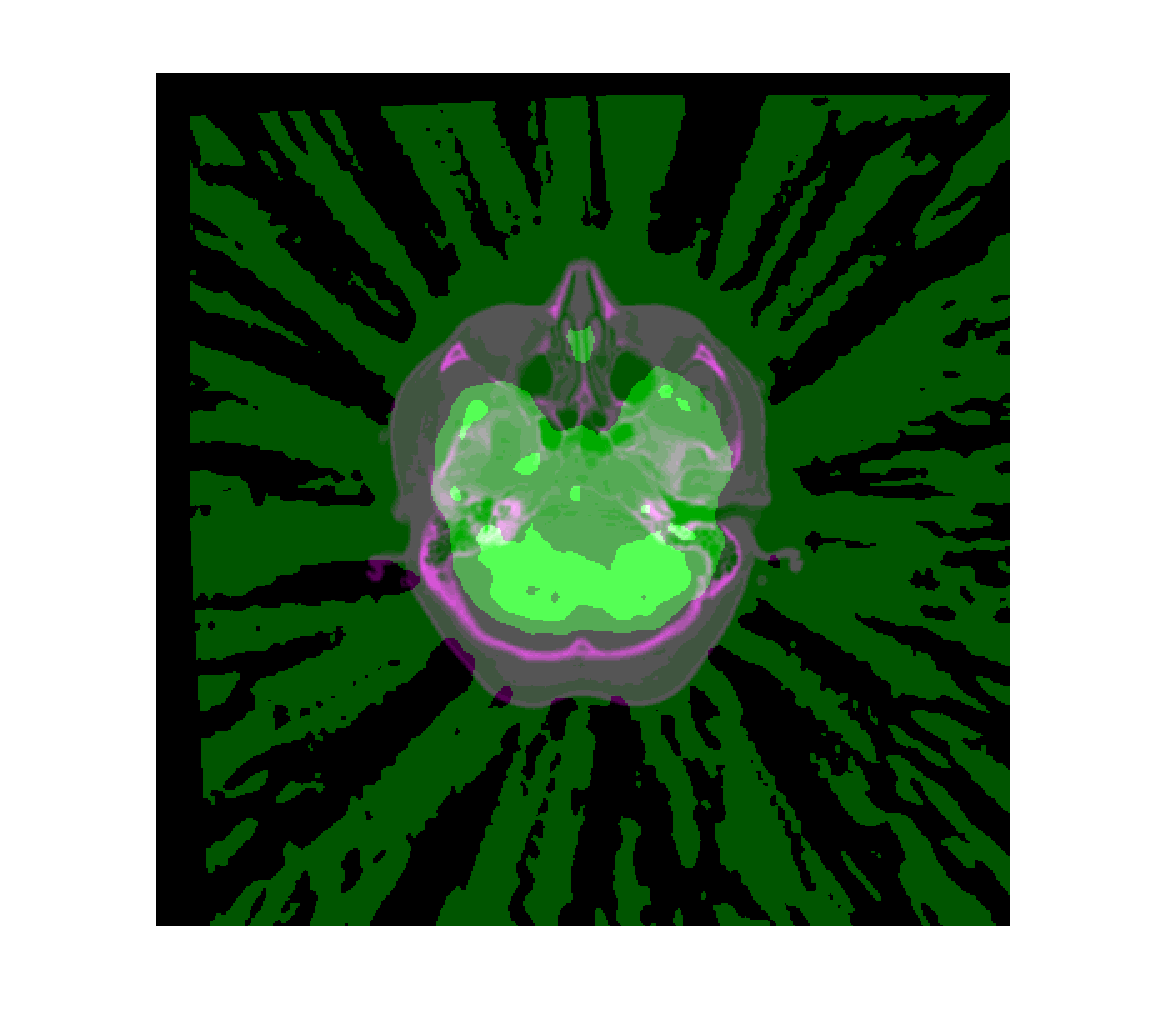
\includegraphics[width=\textwidth]{images/7-reg.eps}
  \caption{Registradas}
\end{figure}
\end{column}
\end{columns}

\end{frame}

% Frame 15
\begin{frame}
\frametitle{IR: Registración en BNCT}

\begin{figure}
  \includegraphics[width=\textwidth]{images/IPTBNCTRegister.png}
\end{figure}

\end{frame}

% Frame 16
\begin{frame}
\frametitle{IR: Software}

\begin{columns}[t]
\column{.5\textwidth}
\pause
\centering
\includegraphics[width=5cm]{images/logos/elastix.png}\\
\pause
\includegraphics[width=5cm]{images/logos/itkLogo.jpg}
\column{.5\textwidth}
\pause
\centering
\includegraphics[width=6cm]{images/logos/opencv.png}\\
\pause
\includegraphics[width=6cm]{images/logos/simpleitk.png}
\end{columns}

\end{frame}

% Frame 17
\begin{frame}
\frametitle{IR: Software}

\hfil\hfil\includegraphics[width=7cm]{images/logos/SimpleElastix.png}\newline
  \null\hfil\hfil\makebox[5cm]{}\newline
  \pause
  \vfil
  \hfil\hfil\includegraphics[width=2cm]{images/logos/c.jpg}\hfil\hfil
    \includegraphics[width=2cm]{images/logos/python.png}\newline
  \null\hfil\hfil\makebox[5cm]{}
    \hfil\hfil\makebox[5cm]{}

\end{frame}

% Frame 18
\begin{frame}
\frametitle{IR}

\begin{block}{}
\centering
\Huge ¿Preguntas?
\end{block}

\end{frame}

% Frame 19
\begin{frame}
\frametitle{IR}

\begin{block}{}
\centering
\Huge ¡Muchas gracias!
\end{block}

\end{frame}


\end{document}
